% ============================================================================
%  Vietnamese Sign Language Recognition using LSTM and MediaPipe
%  Overleaf-ready LaTeX Document
% ============================================================================
\documentclass[12pt, a4paper]{article}

% --- Packages ---
\usepackage[utf8]{inputenc}
\usepackage[T1]{fontenc}
\usepackage{lmodern}
\usepackage[english]{babel}
\usepackage{amsmath, amssymb, amsfonts}
\usepackage{graphicx}
\usepackage{booktabs}
\usepackage{multirow}
\usepackage{caption}
\usepackage{subcaption}
\usepackage{float}
\usepackage{hyperref}
\usepackage{enumitem}
\usepackage{tikz}
\usetikzlibrary{arrows.meta, positioning, shapes.geometric, fit, calc, decorations.pathreplacing}
\usepackage{pgfplots}
\pgfplotsset{compat=1.18}
\usepackage{algorithm}
\usepackage{algpseudocode}
\usepackage{listings}
\usepackage{xcolor}
\usepackage{geometry}
\geometry{margin=2.5cm}
\usepackage{fancyhdr}
\usepackage{setspace}
\onehalfspacing

% --- Hyperref Setup ---
\hypersetup{
    colorlinks=true,
    linkcolor=blue!70!black,
    citecolor=green!50!black,
    urlcolor=blue!60!black,
}

% --- Code listing style ---
\lstset{
    basicstyle=\ttfamily\small,
    keywordstyle=\color{blue}\bfseries,
    commentstyle=\color{gray},
    stringstyle=\color{red!70!black},
    numbers=left,
    numberstyle=\tiny\color{gray},
    frame=single,
    breaklines=true,
    captionpos=b,
}

% --- Header/Footer ---
\pagestyle{fancy}
\fancyhf{}
\fancyhead[L]{\small Vietnamese Sign Language Recognition}
\fancyhead[R]{\small\thepage}
\fancyfoot[C]{\small LSTM + MediaPipe Approach}

% ============================================================================
\begin{document}

% --- Title Page ---
\begin{titlepage}
    \centering
    \vspace*{2cm}
    {\Huge\bfseries Vietnamese Sign Language Recognition\\[0.3cm]
    Using LSTM Neural Network\\[0.3cm]
    and MediaPipe Hand Tracking\par}
    \vspace{1.5cm}
    {\Large A Deep Learning Approach for Real-Time\\
    Gesture Classification\par}
    \vspace{2cm}
    {\large
    \textbf{Author:} Nguyen Thanh Danh\\[0.5cm]
    \textbf{Date:} June 2026\\[0.5cm]
    }
    \vspace{2cm}
    \rule{\textwidth}{0.4pt}\\[0.5cm]
    {\large\itshape
    Keywords: Vietnamese Sign Language, LSTM, MediaPipe, Hand Keypoints,\\
    Deep Learning, Real-Time Recognition, Gesture Classification
    }
    \vfill
\end{titlepage}

% --- Table of Contents ---
\tableofcontents
\newpage

% ============================================================================
% SECTION 1: INTRODUCTION
% ============================================================================
\section{Introduction}
\label{sec:introduction}

\subsection{Problem Statement}

Sign language serves as the primary mode of communication for millions of deaf and hard-of-hearing individuals worldwide. In Vietnam, Vietnamese Sign Language (VSL) is used by approximately 1-2 million people, yet there remains a significant communication barrier between deaf individuals and the hearing population. Unlike spoken languages that can leverage mature speech recognition technology, sign language recognition remains an active and challenging area of research.

The core challenge lies in the \textbf{temporal and spatial complexity} of sign language: each gesture is defined not only by the shape and position of the hand at a single moment (\textit{spatial features}) but also by how the hand moves through a sequence of frames over time (\textit{temporal dynamics}). A robust recognition system must therefore capture both dimensions simultaneously.

\subsection{Objectives}

This project aims to develop a practical, end-to-end system for Vietnamese Sign Language recognition with the following objectives:

\begin{enumerate}[label=(\roman*)]
    \item \textbf{Data Pipeline:} Build an automated pipeline to collect video samples, extract hand keypoints using MediaPipe, and prepare structured datasets for training.
    \item \textbf{Model Training:} Design and train an LSTM-based neural network capable of classifying 33 distinct VSL signs (26 alphabet letters + 4 vowel variants + 3 common phrases).
    \item \textbf{Real-Time Inference:} Deploy the trained model in a web-based application (Streamlit) for live webcam-based sign language recognition.
    \item \textbf{Performance Evaluation:} Achieve a test accuracy exceeding 95\% with robust per-class metrics across all gesture categories.
\end{enumerate}

\subsection{Scope and Contributions}

This work focuses on \textbf{single-hand, isolated sign recognition} — each sign is a self-contained gesture rather than a continuous sentence. The system recognizes 33 classes comprising:

\begin{itemize}
    \item 26 Vietnamese alphabet characters: \texttt{a, aa, aw, b, c, d, dd, e, ee, g, h, i, k, l, m, n, o, oo, ow, p, q, r, s, t, u, uw, v, x, y}
    \item 4 Vietnamese-specific vowel variants: \texttt{aa} (\^a), \texttt{aw} (\u{a}), \texttt{ee} (\^e), \texttt{oo} (\^o), \texttt{ow} (\u{o}), \texttt{uw} (\u{u})
    \item 3 common phrases: \texttt{chao} (hello), \texttt{cam\_on} (thank you), \texttt{ten\_la} (my name is), \texttt{toi} (I/me)
\end{itemize}

% ============================================================================
% SECTION 2: THEORETICAL BACKGROUND
% ============================================================================
\section{Theoretical Background}
\label{sec:theory}

\subsection{Hand Pose Estimation with MediaPipe}

MediaPipe Hands~\cite{mediapipe2020} is a high-fidelity hand tracking solution developed by Google that employs a two-stage detection pipeline:

\begin{enumerate}
    \item \textbf{Palm Detection Model:} A single-shot detector (based on BlazePalm) locates the palm bounding box within the input frame.
    \item \textbf{Hand Landmark Model:} Given the cropped palm region, a regression network predicts 21 3D landmarks (keypoints) representing the skeletal structure of the hand.
\end{enumerate}

Each landmark $\mathbf{p}_i = (x_i, y_i, z_i)$ for $i \in \{0, 1, \ldots, 20\}$ is expressed in normalized image coordinates, where $(x, y) \in [0, 1]$ and $z$ represents relative depth with respect to the wrist.

\begin{figure}[H]
    \centering
    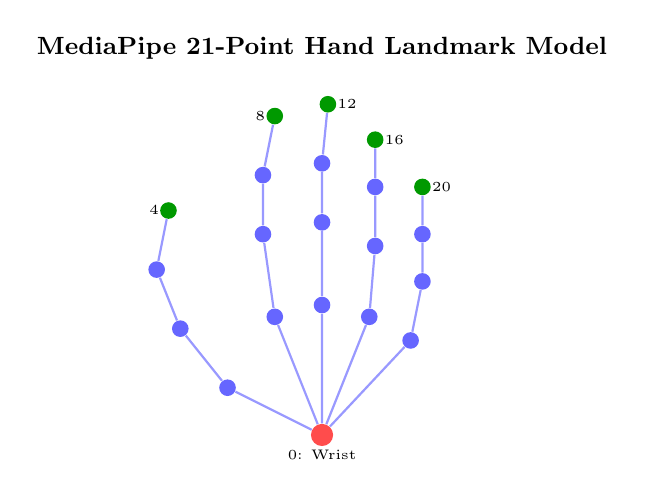
\begin{tikzpicture}[
        joint/.style={circle, fill=blue!60, minimum size=6pt, inner sep=0pt},
        wrist/.style={circle, fill=red!70, minimum size=8pt, inner sep=0pt},
        tip/.style={circle, fill=green!60!black, minimum size=6pt, inner sep=0pt},
        conn/.style={thick, blue!40},
        label/.style={font=\tiny, text=black},
        scale=1.5
    ]
        % Wrist
        \node[wrist] (w) at (0, 0) {};
        \node[label, below=2pt] at (w) {0: Wrist};

        % Thumb
        \node[joint] (t1) at (-0.8, 0.4) {};
        \node[joint] (t2) at (-1.2, 0.9) {};
        \node[joint] (t3) at (-1.4, 1.4) {};
        \node[tip]   (t4) at (-1.3, 1.9) {};
        \draw[conn] (w)--(t1)--(t2)--(t3)--(t4);
        \node[label, left] at (t4) {4};

        % Index
        \node[joint] (i1) at (-0.4, 1.0) {};
        \node[joint] (i2) at (-0.5, 1.7) {};
        \node[joint] (i3) at (-0.5, 2.2) {};
        \node[tip]   (i4) at (-0.4, 2.7) {};
        \draw[conn] (w)--(i1)--(i2)--(i3)--(i4);
        \node[label, left] at (i4) {8};

        % Middle
        \node[joint] (m1) at (0.0, 1.1) {};
        \node[joint] (m2) at (0.0, 1.8) {};
        \node[joint] (m3) at (0.0, 2.3) {};
        \node[tip]   (m4) at (0.05, 2.8) {};
        \draw[conn] (w)--(m1)--(m2)--(m3)--(m4);
        \node[label, right] at (m4) {12};

        % Ring
        \node[joint] (r1) at (0.4, 1.0) {};
        \node[joint] (r2) at (0.45, 1.6) {};
        \node[joint] (r3) at (0.45, 2.1) {};
        \node[tip]   (r4) at (0.45, 2.5) {};
        \draw[conn] (w)--(r1)--(r2)--(r3)--(r4);
        \node[label, right] at (r4) {16};

        % Pinky
        \node[joint] (p1) at (0.75, 0.8) {};
        \node[joint] (p2) at (0.85, 1.3) {};
        \node[joint] (p3) at (0.85, 1.7) {};
        \node[tip]   (p4) at (0.85, 2.1) {};
        \draw[conn] (w)--(p1)--(p2)--(p3)--(p4);
        \node[label, right] at (p4) {20};

        % Title
        \node[font=\small\bfseries, above] at (0, 3.1) {MediaPipe 21-Point Hand Landmark Model};
    \end{tikzpicture}
    \caption{MediaPipe hand landmark topology. The wrist (landmark 0, red) serves as the origin for relative coordinate computation. Fingertips (green) are landmarks 4, 8, 12, 16, 20.}
    \label{fig:hand_landmarks}
\end{figure}

\subsubsection{Relative Coordinate Normalization}

To achieve translation invariance, all keypoints are transformed into a \textbf{wrist-relative coordinate system}. Given wrist position $\mathbf{p}_0 = (x_0, y_0, z_0)$, each landmark is normalized as:

\begin{equation}
    \hat{\mathbf{p}}_i = \mathbf{p}_i - \mathbf{p}_0 = (x_i - x_0,\ y_i - y_0,\ z_i - z_0), \quad i = 0, 1, \ldots, 20
    \label{eq:relative_coords}
\end{equation}

This yields a feature vector of dimensionality $21 \times 3 = 63$ per frame, where $\hat{\mathbf{p}}_0 = (0, 0, 0)$ by construction. The resulting representation is invariant to the absolute position of the hand within the camera frame.

\subsection{Recurrent Neural Networks and LSTM}

\subsubsection{Motivation for Sequential Modeling}

Sign language gestures are inherently \textit{temporal sequences}. A single static frame cannot distinguish between signs that share similar hand shapes but differ in motion trajectory (e.g., different directional movements). Therefore, a model must process an ordered sequence of frames $\mathbf{X} = [\mathbf{x}_1, \mathbf{x}_2, \ldots, \mathbf{x}_T]$, where $T$ is the sequence length and $\mathbf{x}_t \in \mathbb{R}^{63}$ represents the hand keypoints at time step $t$.

\subsubsection{Vanilla RNN Limitations}

A standard Recurrent Neural Network (RNN) maintains a hidden state $\mathbf{h}_t$ that is updated at each time step:

\begin{equation}
    \mathbf{h}_t = \tanh(\mathbf{W}_{hh}\mathbf{h}_{t-1} + \mathbf{W}_{xh}\mathbf{x}_t + \mathbf{b}_h)
    \label{eq:rnn}
\end{equation}

However, vanilla RNNs suffer from the \textbf{vanishing gradient problem}: during backpropagation through time (BPTT), gradients are multiplied by the recurrent weight matrix at each step. For long sequences, these products shrink exponentially, causing the model to fail at capturing long-range temporal dependencies.

\subsubsection{Long Short-Term Memory (LSTM)}

The LSTM architecture~\cite{hochreiter1997lstm} addresses the vanishing gradient problem by introducing a \textbf{cell state} $\mathbf{c}_t$ and three gating mechanisms:

\begin{align}
    \mathbf{f}_t &= \sigma(\mathbf{W}_f [\mathbf{h}_{t-1}, \mathbf{x}_t] + \mathbf{b}_f) & \text{(Forget gate)} \label{eq:forget} \\
    \mathbf{i}_t &= \sigma(\mathbf{W}_i [\mathbf{h}_{t-1}, \mathbf{x}_t] + \mathbf{b}_i) & \text{(Input gate)} \label{eq:input} \\
    \tilde{\mathbf{c}}_t &= \tanh(\mathbf{W}_c [\mathbf{h}_{t-1}, \mathbf{x}_t] + \mathbf{b}_c) & \text{(Candidate cell)} \label{eq:candidate} \\
    \mathbf{c}_t &= \mathbf{f}_t \odot \mathbf{c}_{t-1} + \mathbf{i}_t \odot \tilde{\mathbf{c}}_t & \text{(Cell state update)} \label{eq:cell} \\
    \mathbf{o}_t &= \sigma(\mathbf{W}_o [\mathbf{h}_{t-1}, \mathbf{x}_t] + \mathbf{b}_o) & \text{(Output gate)} \label{eq:output} \\
    \mathbf{h}_t &= \mathbf{o}_t \odot \tanh(\mathbf{c}_t) & \text{(Hidden state)} \label{eq:hidden}
\end{align}

where $\sigma(\cdot)$ is the sigmoid activation function, $\odot$ denotes element-wise (Hadamard) multiplication, and $[\cdot, \cdot]$ represents concatenation.

\begin{figure}[H]
    \centering
    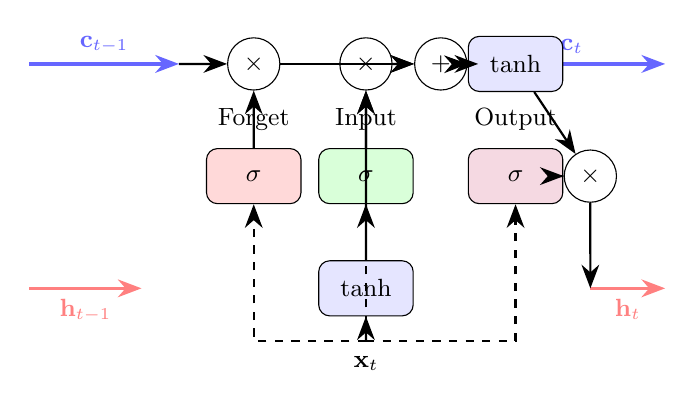
\begin{tikzpicture}[
        gate/.style={rectangle, draw, rounded corners, minimum width=1.2cm, minimum height=0.7cm, fill=yellow!20, font=\small},
        op/.style={circle, draw, minimum size=0.6cm, font=\small},
        arr/.style={-{Stealth[length=3mm]}, thick},
        scale=0.95
    ]
        % Cell state line
        \draw[arr, very thick, blue!60] (-1, 3) -- node[above, font=\small] {$\mathbf{c}_{t-1}$} (1, 3);
        \draw[arr, very thick, blue!60] (5, 3) -- node[above, font=\small] {$\mathbf{c}_{t}$} (7.5, 3);

        % Hidden state line
        \draw[arr, very thick, red!50] (-1, 0) -- node[below, font=\small] {$\mathbf{h}_{t-1}$} (0.5, 0);
        \draw[arr, very thick, red!50] (6.5, 0) -- node[below, font=\small] {$\mathbf{h}_{t}$} (7.5, 0);

        % Forget gate
        \node[gate, fill=red!15] (fg) at (2, 1.5) {$\sigma$};
        \node[font=\small, above=0.1cm] at (fg.north) {Forget};
        \node[op] (fmul) at (2, 3) {$\times$};
        \draw[arr] (fg) -- (fmul);
        \draw[arr] (1, 3) -- (fmul);

        % Input gate
        \node[gate, fill=green!15] (ig) at (3.5, 1.5) {$\sigma$};
        \node[font=\small, above=0.1cm] at (ig.north) {Input};
        \node[gate, fill=blue!10] (cand) at (3.5, 0) {$\tanh$};
        \node[op] (imul) at (3.5, 3) {$\times$};
        \node[op] (add) at (4.5, 3) {$+$};
        \draw[arr] (ig) -- (imul);
        \draw[arr] (cand) -- (imul);
        \draw[arr] (fmul) -- (add);
        \draw[arr] (imul) -- (add);

        % Output gate
        \node[gate, fill=purple!15] (og) at (5.5, 1.5) {$\sigma$};
        \node[font=\small, above=0.1cm] at (og.north) {Output};
        \node[gate, fill=blue!10] (otanh) at (5.5, 3) {$\tanh$};
        \node[op] (omul) at (6.5, 1.5) {$\times$};
        \draw[arr] (add) -- (otanh);
        \draw[arr] (otanh) -- (omul);
        \draw[arr] (og) -- (omul);
        \draw[arr] (omul) -- (6.5, 0);
        \draw[arr] (add) -- (5, 3);

        % Input x_t
        \node[font=\small] at (3.5, -1) {$\mathbf{x}_t$};
        \draw[arr, dashed] (3.5, -0.7) -- (cand);
        \draw[arr, dashed] (3.5, -0.7) -| (fg);
        \draw[arr, dashed] (3.5, -0.7) -| (ig);
        \draw[arr, dashed] (3.5, -0.7) -| (og);
    \end{tikzpicture}
    \caption{Internal architecture of a single LSTM cell. The forget gate controls how much prior cell state to retain, the input gate regulates new information flow, and the output gate modulates the exposed hidden state.}
    \label{fig:lstm_cell}
\end{figure}

\subsection{Classification with Softmax}

The final hidden state $\mathbf{h}_T$ (at the last time step) encodes the entire sequence's temporal representation. This is projected to class logits through a fully connected layer:

\begin{equation}
    \mathbf{z} = \mathbf{W}_{fc} \cdot \mathbf{h}_T + \mathbf{b}_{fc}, \quad \mathbf{z} \in \mathbb{R}^C
    \label{eq:fc}
\end{equation}

where $C = 33$ is the number of gesture classes. The probability distribution over classes is obtained via the softmax function:

\begin{equation}
    P(y = k \mid \mathbf{X}) = \frac{\exp(z_k)}{\sum_{j=1}^{C} \exp(z_j)}, \quad k = 1, \ldots, C
    \label{eq:softmax}
\end{equation}

\subsection{Loss Function: Cross-Entropy}

The model is trained by minimizing the categorical cross-entropy loss:

\begin{equation}
    \mathcal{L} = -\frac{1}{N} \sum_{n=1}^{N} \sum_{k=1}^{C} y_{n,k} \log P(y_n = k \mid \mathbf{X}_n)
    \label{eq:cross_entropy}
\end{equation}

where $N$ is the batch size, $y_{n,k}$ is the one-hot encoded ground truth label, and $P(y_n = k \mid \mathbf{X}_n)$ is the predicted probability for class $k$.

\subsection{Regularization Techniques}

To prevent overfitting on the training data, the following regularization strategies are employed:

\begin{enumerate}
    \item \textbf{Dropout}~\cite{srivastava2014dropout}: During training, random neurons are deactivated with probability $p$. The model uses $p = 0.3$ between LSTM layers and $p = 0.4$ before the final classification layer.

    \item \textbf{Layer Normalization}~\cite{ba2016layernorm}: Applied to the LSTM output to stabilize the distribution of activations, accelerating training convergence.

    \item \textbf{Weight Decay (L2 Regularization):} A penalty term $\lambda \|\mathbf{W}\|_2^2$ with $\lambda = 10^{-4}$ is added to the loss function to discourage large weight magnitudes.

    \item \textbf{Gradient Clipping}: Gradients are clipped to a maximum norm of 1.0 to prevent gradient explosion during BPTT.

    \item \textbf{Data Augmentation}: Random transformations applied to training sequences (see Section~\ref{sec:augmentation}).

    \item \textbf{Early Stopping}: Training is halted when the validation accuracy does not improve for 20 consecutive epochs.
\end{enumerate}


% ============================================================================
% SECTION 3: SYSTEM ARCHITECTURE
% ============================================================================
\section{System Architecture}
\label{sec:architecture}

\subsection{End-to-End Pipeline Overview}

The complete system operates as a five-stage pipeline, from raw video collection to real-time inference:

\begin{figure}[H]
    \centering
    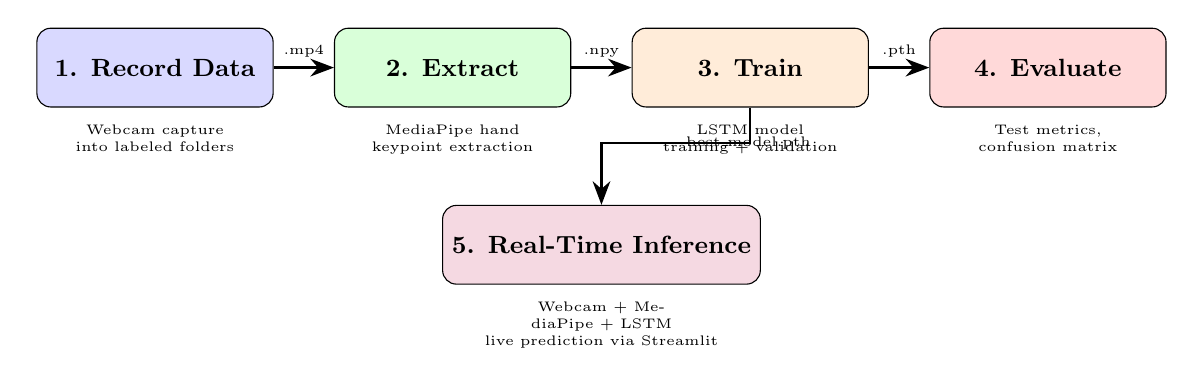
\begin{tikzpicture}[
        block/.style={rectangle, draw, rounded corners=5pt, minimum width=3cm, minimum height=1cm, text centered, font=\small\bfseries},
        arr/.style={-{Stealth[length=3mm]}, thick},
        desc/.style={font=\tiny, text width=3cm, text centered},
        scale=0.9
    ]
        % Stage 1
        \node[block, fill=blue!15] (s1) at (0, 0) {1. Record Data};
        \node[desc, below=0.1cm] at (s1.south) {Webcam capture\\into labeled folders};

        % Stage 2
        \node[block, fill=green!15] (s2) at (4.2, 0) {2. Extract};
        \node[desc, below=0.1cm] at (s2.south) {MediaPipe hand\\keypoint extraction};

        % Stage 3
        \node[block, fill=orange!15] (s3) at (8.4, 0) {3. Train};
        \node[desc, below=0.1cm] at (s3.south) {LSTM model\\training + validation};

        % Stage 4
        \node[block, fill=red!15] (s4) at (12.6, 0) {4. Evaluate};
        \node[desc, below=0.1cm] at (s4.south) {Test metrics,\\confusion matrix};

        % Stage 5
        \node[block, fill=purple!15] (s5) at (6.3, -2.5) {5. Real-Time Inference};
        \node[desc, below=0.1cm] at (s5.south) {Webcam + MediaPipe + LSTM\\live prediction via Streamlit};

        % Arrows
        \draw[arr] (s1) -- node[above, font=\tiny] {.mp4} (s2);
        \draw[arr] (s2) -- node[above, font=\tiny] {.npy} (s3);
        \draw[arr] (s3) -- node[above, font=\tiny] {.pth} (s4);
        \draw[arr] (s3.south) -- ++(0, -0.5) -| node[near start, right, font=\tiny] {best\_model.pth} (s5);
    \end{tikzpicture}
    \caption{End-to-end pipeline of the VSL recognition system.}
    \label{fig:pipeline}
\end{figure}

\subsection{Neural Network Architecture}

The model architecture consists of a stacked 2-layer LSTM followed by Layer Normalization, Dropout, and a fully connected classification head.

\begin{figure}[H]
    \centering
    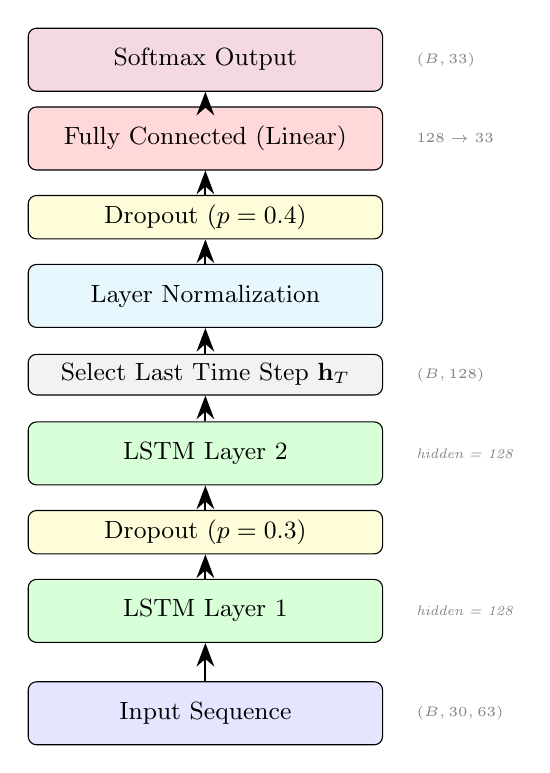
\begin{tikzpicture}[
        layer/.style={rectangle, draw, rounded corners=3pt, minimum width=4.5cm, minimum height=0.8cm, text centered, font=\small},
        arr/.style={-{Stealth[length=3mm]}, thick},
        dim/.style={font=\tiny\itshape, text=gray},
    ]
        % Input
        \node[layer, fill=blue!10] (input) at (0, 0) {Input Sequence};
        \node[dim, right=0.3cm] at (input.east) {$(B, 30, 63)$};

        % LSTM Layer 1
        \node[layer, fill=green!15] (lstm1) at (0, 1.3) {LSTM Layer 1};
        \node[dim, right=0.3cm] at (lstm1.east) {hidden = 128};

        % Dropout between LSTM
        \node[layer, fill=yellow!15, minimum height=0.5cm] (drop1) at (0, 2.3) {Dropout ($p=0.3$)};

        % LSTM Layer 2
        \node[layer, fill=green!15] (lstm2) at (0, 3.3) {LSTM Layer 2};
        \node[dim, right=0.3cm] at (lstm2.east) {hidden = 128};

        % Take last time step
        \node[layer, fill=gray!10, minimum height=0.5cm] (last) at (0, 4.3) {Select Last Time Step $\mathbf{h}_T$};
        \node[dim, right=0.3cm] at (last.east) {$(B, 128)$};

        % Layer Norm
        \node[layer, fill=cyan!10] (ln) at (0, 5.3) {Layer Normalization};

        % Dropout
        \node[layer, fill=yellow!15, minimum height=0.5cm] (drop2) at (0, 6.3) {Dropout ($p=0.4$)};

        % FC
        \node[layer, fill=red!15] (fc) at (0, 7.3) {Fully Connected (Linear)};
        \node[dim, right=0.3cm] at (fc.east) {$128 \to 33$};

        % Output
        \node[layer, fill=purple!15] (out) at (0, 8.3) {Softmax Output};
        \node[dim, right=0.3cm] at (out.east) {$(B, 33)$};

        % Arrows
        \draw[arr] (input) -- (lstm1);
        \draw[arr] (lstm1) -- (drop1);
        \draw[arr] (drop1) -- (lstm2);
        \draw[arr] (lstm2) -- (last);
        \draw[arr] (last) -- (ln);
        \draw[arr] (ln) -- (drop2);
        \draw[arr] (drop2) -- (fc);
        \draw[arr] (fc) -- (out);
    \end{tikzpicture}
    \caption{Model architecture: stacked 2-layer LSTM with Layer Normalization and Dropout regularization. $B$ denotes the batch size.}
    \label{fig:model_arch}
\end{figure}

\subsubsection{Parameter Count}

The total number of trainable parameters is computed as follows. For a single LSTM layer with input size $d$ and hidden size $h$:

\begin{equation}
    \text{Params}_{\text{LSTM}} = 4 \times [(d + h) \times h + h]
    \label{eq:lstm_params}
\end{equation}

The factor of 4 accounts for the four weight matrices (forget, input, candidate, output gates).

\begin{table}[H]
    \centering
    \caption{Breakdown of trainable parameters by layer.}
    \label{tab:params}
    \begin{tabular}{lrr}
        \toprule
        \textbf{Layer} & \textbf{Dimensions} & \textbf{Parameters} \\
        \midrule
        LSTM Layer 1 & $63 \to 128$ & $4 \times [(63+128) \times 128 + 128] = 98{,}304 + 512$ \\
        LSTM Layer 2 & $128 \to 128$ & $4 \times [(128+128) \times 128 + 128] = 131{,}072 + 512$ \\
        Layer Norm   & $128$ & $256$ \\
        FC (Linear)  & $128 \to 33$ & $128 \times 33 + 33 = 4{,}257$ \\
        \midrule
        \textbf{Total} & & $\approx$ \textbf{234{,}913} \\
        \bottomrule
    \end{tabular}
\end{table}

\subsection{Data Augmentation}
\label{sec:augmentation}

To increase the effective training set size and improve model robustness, the following augmentation techniques are applied stochastically during training:

\begin{table}[H]
    \centering
    \caption{Data augmentation strategies applied during training.}
    \label{tab:augmentation}
    \begin{tabular}{llll}
        \toprule
        \textbf{Augmentation} & \textbf{Probability} & \textbf{Parameters} & \textbf{Purpose} \\
        \midrule
        Gaussian Noise & 30\% & $\mu=0, \sigma=0.01$ & Simulate sensor noise \\
        Amplitude Scaling & 30\% & Scale $\in [0.95, 1.05]$ & Hand size variation \\
        Temporal Shift & 20\% & Shift $\in \{-1, 0, +1\}$ & Timing variation \\
        \bottomrule
    \end{tabular}
\end{table}

\subsection{Class Imbalance Handling}

Even with a nearly balanced dataset (61 samples per class), a \textbf{WeightedRandomSampler} is employed during training to ensure every class is equally represented in each epoch:

\begin{equation}
    w_k = \frac{1}{n_k}, \quad \text{where } n_k = \text{number of samples in class } k
    \label{eq:class_weight}
\end{equation}

Each sample is then assigned a weight equal to $w_k$ for its class, and the sampler draws samples with replacement according to these weights.

% ============================================================================
% SECTION 4: DATASET
% ============================================================================
\section{Dataset}
\label{sec:dataset}

\subsection{Data Collection}

Video samples were recorded using a standard USB webcam at 30 FPS with a resolution of $640 \times 480$ pixels. For each of the 33 gesture classes, 61 video clips were recorded, yielding a total of \textbf{2{,}013 samples}.

Each video clip was captured with the following protocol:
\begin{itemize}
    \item The subject positions one hand in front of the camera.
    \item The gesture is performed naturally at conversational speed.
    \item The recording includes approximately 2--3 seconds of footage (60--90 frames).
    \item Frame mirroring (\texttt{cv2.flip}) is applied at recording time for natural visual feedback.
\end{itemize}

\subsection{Keypoint Extraction}

Each video is processed through MediaPipe Hands to extract per-frame keypoints:

\begin{enumerate}
    \item Each frame is resized to $640 \times 480$ and converted from BGR to RGB.
    \item MediaPipe Hands detects the hand and returns 21 3D landmarks.
    \item Coordinates are transformed to wrist-relative using Equation~\eqref{eq:relative_coords}.
    \item The resulting 63-dimensional feature vector is stored for each frame.
\end{enumerate}

\subsubsection{Sequence Normalization}

Since videos have varying lengths, all sequences are normalized to a fixed length $T = 30$ frames:

\begin{itemize}
    \item \textbf{If $L > T$:} Uniform temporal sampling using $T$ evenly spaced indices: $\text{idx}_i = \lfloor i \cdot (L-1) / (T-1) \rfloor$.
    \item \textbf{If $L < T$:} Zero-padding is appended to fill the remaining frames.
    \item \textbf{If $L = T$:} The sequence is used as-is.
\end{itemize}

The final keypoint data for each sample is stored as a NumPy array of shape $(30, 63)$.

\subsection{Dataset Statistics}

\begin{table}[H]
    \centering
    \caption{Summary of the VSL dataset.}
    \label{tab:dataset_stats}
    \begin{tabular}{lr}
        \toprule
        \textbf{Property} & \textbf{Value} \\
        \midrule
        Total samples & 2{,}013 \\
        Number of classes & 33 \\
        Samples per class & 61 (balanced) \\
        Sequence length $T$ & 30 frames \\
        Feature dimension & 63 (21 landmarks $\times$ 3 coords) \\
        Input tensor shape & $(30, 63)$ \\
        \bottomrule
    \end{tabular}
\end{table}

\subsection{Train / Validation / Test Split}

The dataset is divided using \textbf{Stratified Shuffle Split} to ensure proportional class representation in each subset:

\begin{table}[H]
    \centering
    \caption{Dataset split configuration and resulting sizes.}
    \label{tab:split}
    \begin{tabular}{lcr}
        \toprule
        \textbf{Subset} & \textbf{Ratio} & \textbf{Samples} \\
        \midrule
        Training   & 80\% & 1{,}609 \\
        Validation & 10\% & 202 \\
        Test       & 10\% & 202 \\
        \midrule
        \textbf{Total} & 100\% & \textbf{2{,}013} \\
        \bottomrule
    \end{tabular}
\end{table}

% ============================================================================
% SECTION 5: TRAINING
% ============================================================================
\section{Training Methodology}
\label{sec:training}

\subsection{Hyperparameter Configuration}

\begin{table}[H]
    \centering
    \caption{Training hyperparameters.}
    \label{tab:hyperparams}
    \begin{tabular}{lll}
        \toprule
        \textbf{Hyperparameter} & \textbf{Value} & \textbf{Rationale} \\
        \midrule
        Optimizer & Adam & Adaptive learning rate per parameter \\
        Learning Rate & $1 \times 10^{-3}$ & Standard for Adam with batch size 16 \\
        Weight Decay ($\lambda$) & $1 \times 10^{-4}$ & L2 regularization to prevent overfitting \\
        Batch Size & 16 & Stable gradient estimates for $\sim$2000 samples \\
        Max Epochs & 150 & Upper bound; early stopping typically triggers \\
        Early Stopping Patience & 20 epochs & Prevents premature termination \\
        LR Scheduler & ReduceLROnPlateau & Halves LR after 7 epochs of no val\_loss improvement \\
        Gradient Clipping & max\_norm = 1.0 & Prevents gradient explosion in BPTT \\
        Random Seed & 42 & Ensures reproducibility \\
        \bottomrule
    \end{tabular}
\end{table}

\subsection{Learning Rate Schedule}

The learning rate is adjusted dynamically using \texttt{ReduceLROnPlateau}:

\begin{equation}
    \text{lr}_{\text{new}} = \text{lr}_{\text{old}} \times \gamma, \quad \gamma = 0.5
    \label{eq:lr_schedule}
\end{equation}

This reduction is triggered when the validation loss does not decrease for 7 consecutive epochs. The observed LR trajectory during training was:

\begin{center}
    $10^{-3} \xrightarrow{\text{epoch 47}} 5 \times 10^{-4} \xrightarrow{\text{epoch 69}} 2.5 \times 10^{-4} \xrightarrow{\text{epoch 79}} 1.25 \times 10^{-4}$
\end{center}

\subsection{Training Algorithm}

\begin{algorithm}[H]
    \caption{Training Procedure with Early Stopping}
    \label{alg:training}
    \begin{algorithmic}[1]
        \Require Training set $\mathcal{D}_{\text{train}}$, Validation set $\mathcal{D}_{\text{val}}$, Patience $P=20$
        \State Initialize model weights randomly
        \State $\text{best\_acc} \gets 0$, $\text{epochs\_no\_improve} \gets 0$
        \For{$e = 1$ to $E_{\max}$}
            \For{each mini-batch $(\mathbf{X}, \mathbf{y})$ in $\mathcal{D}_{\text{train}}$}
                \State $\hat{\mathbf{X}} \gets \text{Augment}(\mathbf{X})$ \Comment{Apply random augmentation}
                \State $\hat{\mathbf{y}} \gets \text{Model}(\hat{\mathbf{X}})$ \Comment{Forward pass}
                \State $\mathcal{L} \gets \text{CrossEntropy}(\hat{\mathbf{y}}, \mathbf{y})$
                \State Compute $\nabla \mathcal{L}$ via BPTT
                \State Clip gradients: $\|\nabla\| \leq 1.0$
                \State Update weights via Adam
            \EndFor
            \State $\text{val\_acc} \gets \text{Evaluate}(\text{Model}, \mathcal{D}_{\text{val}})$
            \If{$\text{val\_acc} > \text{best\_acc}$}
                \State $\text{best\_acc} \gets \text{val\_acc}$
                \State Save model checkpoint
                \State $\text{epochs\_no\_improve} \gets 0$
            \Else
                \State $\text{epochs\_no\_improve} \gets \text{epochs\_no\_improve} + 1$
            \EndIf
            \If{$\text{epochs\_no\_improve} \geq P$}
                \State \textbf{break} \Comment{Early stopping}
            \EndIf
            \State Update learning rate (ReduceLROnPlateau)
        \EndFor
    \end{algorithmic}
\end{algorithm}

% ============================================================================
% SECTION 6: EXPERIMENTAL RESULTS
% ============================================================================
\section{Experimental Results}
\label{sec:results}

\subsection{Training Convergence}

The model was trained for 90 epochs before early stopping was triggered. Figure~\ref{fig:training_curves} shows the convergence of loss and accuracy across training and validation sets.

\begin{figure}[H]
    \centering
    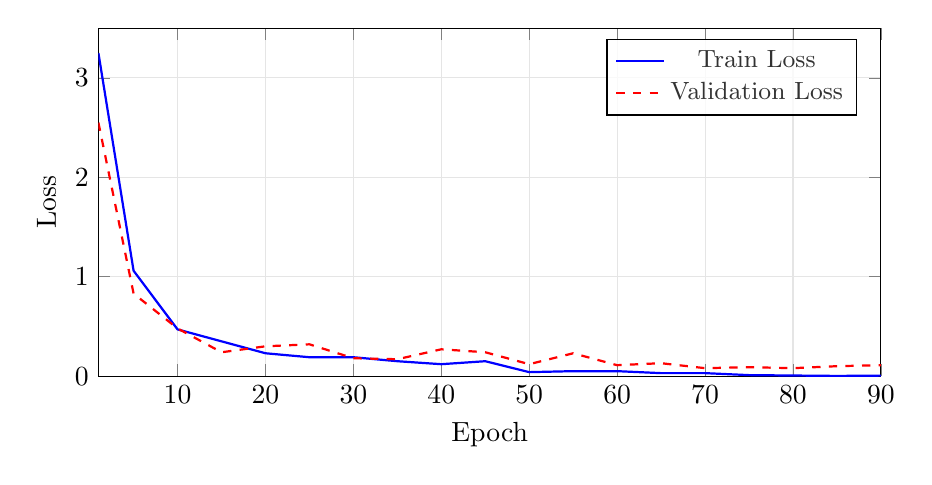
\begin{tikzpicture}
        \begin{axis}[
            width=0.95\textwidth,
            height=6cm,
            xlabel={Epoch},
            ylabel={Loss},
            legend pos=north east,
            grid=major,
            grid style={gray!20},
            xmin=1, xmax=90,
            ymin=0, ymax=3.5,
            legend style={font=\small, fill=white, fill opacity=0.8},
        ]
            % Train Loss (sampled key points)
            \addplot[blue, thick, mark=none] coordinates {
                (1,3.25) (5,1.06) (10,0.47) (15,0.35) (20,0.23)
                (25,0.19) (30,0.19) (35,0.15) (40,0.12) (45,0.15)
                (50,0.04) (55,0.05) (60,0.05) (65,0.03) (70,0.03)
                (75,0.01) (80,0.006) (85,0.002) (90,0.005)
            };
            \addlegendentry{Train Loss}

            % Val Loss (sampled key points)
            \addplot[red, thick, dashed, mark=none] coordinates {
                (1,2.55) (5,0.83) (10,0.48) (15,0.24) (20,0.30)
                (25,0.32) (30,0.18) (35,0.17) (40,0.27) (45,0.24)
                (50,0.12) (55,0.23) (60,0.11) (65,0.13) (70,0.08)
                (75,0.09) (80,0.08) (85,0.10) (90,0.11)
            };
            \addlegendentry{Validation Loss}
        \end{axis}
    \end{tikzpicture}

    \vspace{0.5cm}

    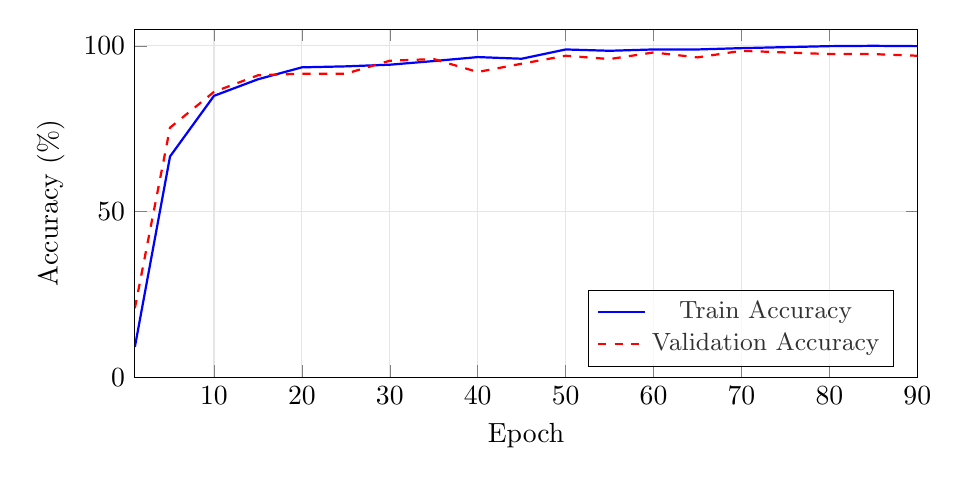
\begin{tikzpicture}
        \begin{axis}[
            width=0.95\textwidth,
            height=6cm,
            xlabel={Epoch},
            ylabel={Accuracy (\%)},
            legend pos=south east,
            grid=major,
            grid style={gray!20},
            xmin=1, xmax=90,
            ymin=0, ymax=105,
            legend style={font=\small, fill=white, fill opacity=0.8},
        ]
            % Train Accuracy
            \addplot[blue, thick, mark=none] coordinates {
                (1,9.1) (5,66.6) (10,84.9) (15,89.9) (20,93.5)
                (25,93.8) (30,94.3) (35,95.4) (40,96.6) (45,96.1)
                (50,98.9) (55,98.5) (60,98.9) (65,98.9) (70,99.3)
                (75,99.6) (80,99.9) (85,100) (90,99.9)
            };
            \addlegendentry{Train Accuracy}

            % Val Accuracy
            \addplot[red, thick, dashed, mark=none] coordinates {
                (1,20.8) (5,75.3) (10,86.1) (15,91.1) (20,91.6)
                (25,91.6) (30,95.5) (35,96.0) (40,92.1) (45,94.6)
                (50,97.0) (55,96.0) (60,98.0) (65,96.5) (70,98.5)
                (75,98.0) (80,97.5) (85,97.5) (90,97.0)
            };
            \addlegendentry{Validation Accuracy}
        \end{axis}
    \end{tikzpicture}
    \caption{Training and validation curves. \textbf{Top:} Loss convergence showing smooth decrease with LR reductions at epochs 47, 69, and 79. \textbf{Bottom:} Accuracy convergence reaching 98.51\% validation accuracy at epoch 70.}
    \label{fig:training_curves}
\end{figure}

\textbf{Key observations:}
\begin{itemize}
    \item Rapid initial convergence: the model reaches $>$90\% validation accuracy by epoch 15.
    \item The LR reduction at epoch 47 ($10^{-3} \to 5 \times 10^{-4}$) triggers a significant jump in training accuracy from $\sim$96\% to $>$99\%.
    \item Best validation accuracy of \textbf{98.51\%} is achieved at epoch 70.
    \item Training accuracy reaches 100\% by epoch 82, indicating the model has fully memorized the training data; however, validation accuracy remains stable at $\sim$97--98\%, suggesting acceptable generalization.
\end{itemize}

\subsection{Test Set Performance}

The best model checkpoint (epoch 70) was evaluated on the held-out test set of 202 samples:

\begin{table}[H]
    \centering
    \caption{Overall test set metrics.}
    \label{tab:overall_metrics}
    \begin{tabular}{lr}
        \toprule
        \textbf{Metric} & \textbf{Value} \\
        \midrule
        Test Accuracy & \textbf{96.04\%} \\
        Macro Precision & 97.44\% \\
        Macro Recall & 96.03\% \\
        Macro F1-Score & 95.93\% \\
        Number of Test Samples & 202 \\
        \bottomrule
    \end{tabular}
\end{table}

\subsection{Per-Class Classification Report}

Table~\ref{tab:per_class} presents the detailed precision, recall, and F1-score for each gesture class.

\begin{table}[H]
    \centering
    \caption{Per-class precision, recall, and F1-score on the test set. Classes with F1 $<$ 1.00 are highlighted.}
    \label{tab:per_class}
    \small
    \begin{tabular}{lcccc}
        \toprule
        \textbf{Class} & \textbf{Precision} & \textbf{Recall} & \textbf{F1-Score} & \textbf{Support} \\
        \midrule
        a      & 0.857 & 1.000 & 0.923 & 6 \\
        aa     & 1.000 & 0.833 & 0.909 & 6 \\
        aw     & 1.000 & 1.000 & 1.000 & 6 \\
        b      & 1.000 & 1.000 & 1.000 & 6 \\
        c      & 1.000 & 1.000 & 1.000 & 6 \\
        cam\_on & 1.000 & 1.000 & 1.000 & 6 \\
        chao   & 1.000 & 1.000 & 1.000 & 6 \\
        d      & 1.000 & 1.000 & 1.000 & 7 \\
        dd     & 0.857 & 1.000 & 0.923 & 6 \\
        e--t   & \multicolumn{4}{c}{\textit{(All 1.000 --- perfect classification)}} \\
        toi    & 0.857 & 1.000 & 0.923 & 6 \\
        \textbf{u} & \textbf{0.583} & \textbf{1.000} & \textbf{0.737} & 7 \\
        uw     & 1.000 & 0.833 & 0.909 & 6 \\
        \textbf{v} & \textbf{1.000} & \textbf{0.333} & \textbf{0.500} & 6 \\
        x      & 1.000 & 1.000 & 1.000 & 6 \\
        y      & 1.000 & 0.833 & 0.909 & 6 \\
        \bottomrule
    \end{tabular}
\end{table}

\subsection{Error Analysis}

The weakest performing classes are:

\begin{enumerate}
    \item \textbf{Class ``v'' (F1 = 0.500):} Only 2 out of 6 test samples were correctly classified (recall = 33.3\%). This is likely caused by visual similarity between the ``v'' sign and other signs like ``u''. The ``v'' gesture (two fingers apart) can be confused when finger separation is not clearly captured.

    \item \textbf{Class ``u'' (F1 = 0.737):} While recall is perfect (100\%), precision is low (58.3\%), meaning the model over-predicts ``u'' — likely absorbing misclassified ``v'' samples.

    \item \textbf{Classes ``a'', ``dd'', ``toi'' (F1 $\approx$ 0.92):} Minor confusion due to similar hand shapes.
\end{enumerate}

\textbf{Potential improvements:}
\begin{itemize}
    \item Collect additional training samples specifically for confusable pairs (u/v, a/dd).
    \item Implement attention mechanisms to focus on discriminative finger positions.
    \item Consider multi-scale temporal features to capture fine-grained motion differences.
\end{itemize}

% ============================================================================
% SECTION 7: REAL-TIME INFERENCE
% ============================================================================
\section{Real-Time Inference System}
\label{sec:realtime}

\subsection{Inference Pipeline}

The real-time recognition system operates as a sliding-window pipeline:

\begin{enumerate}
    \item \textbf{Frame Capture:} Webcam frames are captured at $\sim$30 FPS and horizontally flipped (mirrored view).
    \item \textbf{Hand Detection:} Each frame is processed by MediaPipe Hands (up to 2 hands).
    \item \textbf{Feature Buffer:} Wrist-relative keypoints (63-dim) are appended to a fixed-size buffer of length $T = 30$.
    \item \textbf{Quality Gate:} Prediction is only triggered when $\geq 60\%$ of frames in the buffer contain a detected hand (i.e., at least 18 of 30 frames).
    \item \textbf{Model Inference:} The buffer is converted to a tensor and passed through the LSTM model.
    \item \textbf{Confidence Threshold:} Only predictions with softmax confidence $\geq 75\%$ are displayed to the user.
\end{enumerate}

\subsection{Web Interface}

The application is built using Streamlit and provides:
\begin{itemize}
    \item Live camera feed with hand landmark overlay
    \item Real-time prediction display with confidence percentage
    \item Action history log with temporal grouping
    \item Training management (extract, train, evaluate) via the web UI
    \item Interactive evaluation charts (Plotly-based confusion matrix, per-class metrics)
    \item Bilingual support (Vietnamese / English)
\end{itemize}

% ============================================================================
% SECTION 8: CONCLUSION
% ============================================================================
\section{Conclusion}
\label{sec:conclusion}

This project successfully developed an end-to-end Vietnamese Sign Language recognition system that achieves \textbf{96.04\% test accuracy} across 33 gesture classes using a lightweight LSTM architecture ($\sim$235K parameters). Key accomplishments include:

\begin{enumerate}
    \item A fully automated data pipeline from webcam recording to model deployment.
    \item Effective use of MediaPipe's 21-point hand landmark model for pose-based feature extraction, achieving translation invariance through wrist-relative normalization.
    \item A 2-layer LSTM with regularization techniques (dropout, layer normalization, weight decay, data augmentation) that generalizes well despite a relatively small dataset of 2{,}013 samples.
    \item A production-ready web application for real-time sign language recognition with quality gates and confidence thresholds.
\end{enumerate}

\subsection{Limitations and Future Work}

\begin{itemize}
    \item \textbf{Confusion between similar signs:} The ``u'' and ``v'' pair shows significant confusion (F1 = 0.50 for ``v''). Collecting more diverse training data and exploring attention-based architectures could mitigate this.
    \item \textbf{Single-hand only:} The current system processes only one hand. Extending to two-hand signs would expand the recognizable vocabulary.
    \item \textbf{Isolated signs only:} Continuous sign language recognition (sentence-level) using CTC or Transformer architectures remains as future work.
    \item \textbf{User independence:} The model is trained on data from a single signer. Multi-user datasets would improve generalization.
    \item \textbf{Alternative architectures:} Transformer-based models (e.g., Temporal Convolutional Networks, Vision Transformers) may capture longer-range dependencies more effectively than LSTMs.
\end{itemize}

% ============================================================================
% REFERENCES
% ============================================================================
\begin{thebibliography}{99}

\bibitem{hochreiter1997lstm}
S.~Hochreiter and J.~Schmidhuber,
``Long Short-Term Memory,''
\textit{Neural Computation}, vol.~9, no.~8, pp.~1735--1780, 1997.

\bibitem{mediapipe2020}
F.~Zhang, V.~Bazarevsky, A.~Vakunov, A.~Tkachenka, G.~Sung, C.-L.~Chang, and M.~Grundmann,
``MediaPipe Hands: On-device Real-time Hand Tracking,''
\textit{arXiv preprint arXiv:2006.10214}, 2020.

\bibitem{srivastava2014dropout}
N.~Srivastava, G.~Hinton, A.~Krizhevsky, I.~Sutskever, and R.~Salakhutdinov,
``Dropout: A Simple Way to Prevent Neural Networks from Overfitting,''
\textit{Journal of Machine Learning Research}, vol.~15, pp.~1929--1958, 2014.

\bibitem{ba2016layernorm}
J.~L.~Ba, J.~R.~Kiros, and G.~E.~Hinton,
``Layer Normalization,''
\textit{arXiv preprint arXiv:1607.06450}, 2016.

\bibitem{kingma2015adam}
D.~P.~Kingma and J.~Ba,
``Adam: A Method for Stochastic Optimization,''
\textit{Proceedings of the 3rd International Conference on Learning Representations (ICLR)}, 2015.

\bibitem{luong2015attention}
M.-T.~Luong, H.~Pham, and C.~D.~Manning,
``Effective Approaches to Attention-based Neural Machine Translation,''
\textit{Proceedings of the 2015 Conference on Empirical Methods in Natural Language Processing}, pp.~1412--1421, 2015.

\bibitem{ioffe2015batchnorm}
S.~Ioffe and C.~Szegedy,
``Batch Normalization: Accelerating Deep Network Training by Reducing Internal Covariate Shift,''
\textit{Proceedings of the 32nd International Conference on Machine Learning (ICML)}, pp.~448--456, 2015.

\bibitem{graves2012sequence}
A.~Graves,
``Supervised Sequence Labelling with Recurrent Neural Networks,''
\textit{Studies in Computational Intelligence}, vol.~385, Springer, 2012.

\bibitem{loshchilov2019decoupled}
I.~Loshchilov and F.~Hutter,
``Decoupled Weight Decay Regularization,''
\textit{Proceedings of the 7th International Conference on Learning Representations (ICLR)}, 2019.

\end{thebibliography}

\end{document}
